\chapter{AI in Medicina}
\label{ch:capitolo1}

% --- Inizio del Capitolo 1 ---



\section{Introduzione}
L'integrazione dell'AI nel mondo della medicina rappresenta un punto di svolta nella storia sanitaria. L'AI è ormai utilizzata in una vasta gamma di settori, ma è nel campo medico che si sta assistendo a sviluppi sempre più importanti e significativi. La sua capacità di analizzare enormi quantità di dati, individuare pattern e fornire previsioni accurate sta rivoluzionando la diagnosi, il trattamento e la gestione delle malattie. Le AI sono in grado di aiutare o a volte superare le capacità umane nella precisione diagnostica, come dimostrato da studi che hanno evidenziato l'efficacia degli algoritmi di AI nella diagnosi di condizioni come la retinopatia diabetica\cite{articolo1_retinopatia}\cite{articolo2_retinopatia} e i tumori al seno \cite{articolo1_breastcancer} \cite{articolo2_breastcancer}.
Merita inoltre menzione il recente Modello di Google "MedPalm2", capace  di raggiungere un'accuratezza dell'85.4\% alle domande dell'USMLE(US Medical License Exam), con prestazioni quindi pari a quella di esaminatori "esperti".
\cite{GoogleMedpalm2}

\section{Dati nell'Healthcare}

L'industria del settore medico genera una quantità considerevole di dati ogni giorno, aprendo la strada a un futuro in cui l'IoMT (Internet of Medical Things) diventerà una realtà tangibile. Grazie alla crescente interconnessione tra dispositivi e applicazioni avanzate, i pazienti avranno a disposizione strumenti ad alta funzionalità che consentiranno la generazione, la raccolta, l'analisi e la trasmissione dei dati sanitari. Già oggi, dispositivi come smartwatch, saturimetri e glucometri smart offrono la possibilità di ricevere previsioni sullo stato di salute dei pazienti. Ad esempio, aziende come Samsung \cite{Samsung} e Apple \cite{Apple}, nel 2017, hanno sviluppato algoritmi di deep learning per i loro smartwatch, che sono in grado di rilevare la fibrillazione atriale tramite un monitor ECG e la misurazione del battito cardiaco. Queste innovazioni consentono di individuare precocemente anomalie cardiache e migliorare la gestione delle condizioni di salute.


\begin{figure}[h]
    \centering
    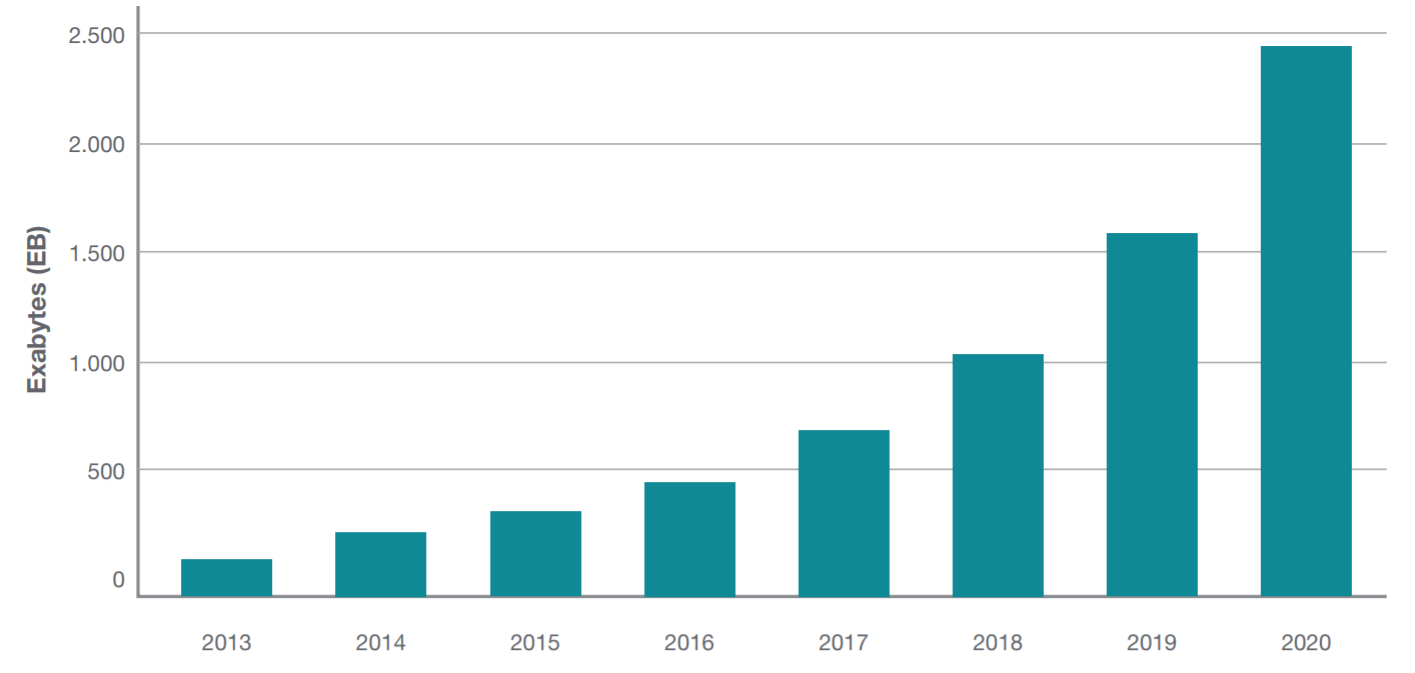
\includegraphics[scale=0.5]{TemplateTesi/immagini/healthcare-data-growth.png}
    
    \caption{Quantità di dati clinici prodotti annualmente dal 2013 al 2020 \cite{crescitadaticlinici}}
    \label{fig:my_label}
\end{figure}
%
%\section{Dati Sintetici Clinici}
%%In ambito medico, l'uso dei dati sintetici, definiti come dati generati a partire da dati reali che mantengono le stesse proprietà statistiche, è fondamentale per affrontare le sfide legate alla privacy e alla sicurezza dei dati sensibili dei pazienti. L'obiettivo principale nell'utilizzo dei dati sintetici è garantire la "utility" dei dati generati, ovvero la misura con cui questi dati sintetici mantengono la somiglianza con i dati reali.\newline
\begin{flushleft}
%%L'accesso ai dati, soprattutto in Europa, può essere spesso problematico a causa delle stringenti politiche sulla privacy e dei costi associati alla raccolta dei dati. 
%%Il processo di raccolta dei dati reali può essere oneroso, limitando la disponibilità di dati completi o utilizzabili.
%%%Questa sfida evidenzia l'importanza dei dati sintetici come alternativa, in quanto consentono di superare le restrizioni legate alla raccolta e all'accesso ai dati reali, fornendo una risorsa preziosa per l'analisi e la ricerca. Questo consente agli scienziati e ai ricercatori di esplorare diversi scenari senza dover accedere direttamente ai dati reali dei pazienti, il tutto senza compromettere la riservatezza dei pazienti. 
%%%Ciò apre nuove opportunità per studiare rare condizioni mediche, valutare l'efficacia di nuovi trattamenti e predire gli esiti delle terapie.



%I modelli basati su dati sintetici consentono di superare le limitazioni associate alla disponibilità di dati reali, consentendo ai ricercatori di addestrare e raffinare algoritmi di AI su dataset più ampi e diversificati. Questo porta a una maggiore precisione nelle previsioni e nelle diagnosi, migliorando l'efficacia complessiva del servizio.
%%\end{figure}



 %La generazione di dati sintetici, o \emph{sintesi}, si basa,come illustrato in  
 %Figura~\ref{fig:synthData}, sull'utilizzo dei dati reali come punto di partenza. 
 %Questo processo coinvolge una serie di passaggi chiave, il primo dei quali è denominato "data preparation". 
 %Durante questa fase, vengono applicate diverse tecniche, tra cui:
%\begin{itemize}
    %\item Data Cleaning: un'operazione volta a rimuovere eventuali errori o inconsistenze presenti nei dati reali
%\item Data Standardization: un processo che mira a organizzare i dati secondo gli stessi schemi di formattazione e struttura
    %\item Data Harmonization: un'attività che si occupa di uniformare i dati provenienti da fonti diverse, allineandoli sotto la stessa categoria

%\end{itemize}

%Una volta completate queste operazioni di preparazione dei dati, si procede alla fase di "Data Synthesis", in cui i dati sintetici vengono generati come risultato finale del processo. 



\end{flushleft}



\section{eHealth: Motivazioni e Campi di utilizzo}
Nell'ambito dell'eHealth, che si riferisce all'utilizzo dell'informatica e della telecomunicazione nel campo della salute,
è fondamentale comprendere il motivo per cui gli sviluppi nel campo delle AI nel settore medico stiano raggiungendo risultati così promettenti,dobbiamo quindi porci le  seguenti domande chiave: 
\begin{itemize}
    \item Perché queste tecnologie sono così importanti nell'healthcare ?
    \item Quali sono le macro aree di applicazione delle AI nel settore medico?
\end{itemize}  
Nelle sezioni sottostanti proverò a dare delle risposte a questi quesiti.


\subsection{Motivazioni}

\begin{itemize}
    \item \textbf{Managing del tempo dello staff medico:}

    Nel campo della sanità, una gestione più efficace del tempo non solo offre un maggiore respiro al personale medico, consentendo loro di concentrarsi su attività di maggior valore, ma contribuisce anche a stabilire un rapporto più forte tra medico e paziente. Diversi studi\cite{RelazionePazienteDoc1}\cite{RelazionePazienteDoc2} hanno dimostrato che una comunicazione migliore e un'attenzione personalizzata da parte del personale medico possono portare a numerosi benefici sulla qualità della cura sottoposta.
    Uno studio rilevante\cite{TempoMedici} sull'impiego del tempo del personale medico ha evidenziato che, il 40\% del loro tempo viene trascorso nella sala dei medici, mentre solo il 14.7\% del tempo è dedicato all'interazione diretta con i pazienti. In questo contesto, l'impiego delle intelligenze artificiali nel managing del tempo dello staff medico assume un ruolo fondamentale. Attraverso l'adozione di soluzioni basate sull'AI, è possibile ridurre i tempi di attesa dei pazienti, ottimizzare la pianificazione delle visite e dei trattamenti, nonché garantire che il personale medico abbia il tempo adeguato per interagire con i pazienti in modo più empatico e approfondito.
    Un esempio in tale campo si può osservare nel progetto appartenente a Dedalus chiamato Clinical Management System (CMS).
    Anche grazie alle AI il sistema CMS è capace di facilitare il managing di reparti chirurgici, accellerando i tempi di attesa, migliorando le qualità delle cure e alleggerendo il carico dello staff medico.\cite{CMSDedalus}
    \newline
    \newline
    \item \textbf{Monitoring da remoto del paziente:}

     Il monitoraggio dei dati in tempo reale nei pazienti riveste un ruolo di fondamentale importanza per la valutazione continua delle condizioni di salute, il rilevamento precoce di eventuali anomalie e la personalizzazione dei trattamenti. In questo contesto, l'impiego delle intelligenze artificiali rappresenta un elemento di grande rilevanza per garantire un monitoraggio accurato e tempestivo dei pazienti\cite{MonitorAI}.
     Grazie alla capacità di elaborare in modo rapido e accurato i dati provenienti da diverse fonti, come sensori indossabili, dispositivi di monitoraggio elettronico e registrazioni cliniche, le AI possono generare modelli predittivi e algoritmi di apprendimento automatico che permettono di adattare i protocolli terapeutici in tempo reale, ottimizzando i risultati clinici e la gestione delle risorse sanitarie,casistica in cui ricade il lavoro che ho svolto presso Dedalus.
     
    \item \textbf{Offrire una nuova prospettiva:} 

    Nel settore clinico le AI sono in grado di superare le limitazioni della visione umana e offrire una prospettiva più ampia. 
    Mentre un medico si basa principalmente sui suoi studi e sull'esperienza personale per formulare diagnosi e piani di trattamento, l'AI può analizzare una vasta quantità di dati provenienti da diverse fonti, inclusi dati clinici, storici dei pazienti, risultati di test di laboratorio e letteratura medica.

    La visione di un medico è intrinsecamente limitata dal tempo a disposizione per studiare e approfondire ogni aspetto della medicina. Tuttavia, le intelligenze artificiali non sono soggette a queste restrizioni e possono elaborare enormi quantità di dati in tempi molto più brevi.
    
    L'AI può supportare i medici nella diagnosi precoce di malattie \cite{articolo1_retinopatia}, fornendo suggerimenti basati su evidenze scientifiche e confrontando i dati dei pazienti con casi simili presenti nella letteratura medica. Questo permette di evitare errori diagnostici e migliorare l'accuratezza delle diagnosi, facendo risparmiare alle strutture sanitarie risorse impiegabili per migliorare la qualità dei loro servizi.
    \item \textbf{Spinta al raccoglimento dei dati e alla digitalizzazione:}

    Le AI offrono un'opportunità per migliorare la gestione dei dati clinici, consentendo la raccolta, l'elaborazione e l'analisi efficiente di enormi quantità di informazioni.

    L'adozione delle AI promuove la digitalizzazione delle pratiche sanitarie. L'implementazione di registri elettronici dei pazienti, sistemi di prescrizione elettronica e piattaforme di telemedicina consente una gestione più efficiente dei dati e una migliore comunicazione tra  sanitari. 

    La digitalizzazione dei dati nel settore clinico ha numerosi vantaggi. Permette un accesso rapido alle informazioni, riduce gli errori di trascrizione, facilita la condivisione sicura dei dati tra diversi operatori sanitari e favorisce la collaborazione interdisciplinare. Inoltre, l'elaborazione automatizzata dei dati consente l'identificazione di pattern e correlazioni che possono contribuire a una migliore comprensione delle malattie e dei trattamenti più efficaci.
\end{itemize}

\subsection{Campi di Utilizzo}

\begin{itemize}
    \item \textbf{Personalizzazione delle cure:}

    
    le AI possono analizzare e interpretare informazioni dettagliate sui pazienti, come il loro background medico, le condizioni di salute preesistenti, i risultati dei test di laboratorio e i dati genetici.
    Sono quindi in grado di identificare pattern e correlazioni tra i dati, consentendo ai medici di prendere decisioni basate su informazioni più accurate e specifiche per ogni paziente. Questo approccio personalizzato può portare a numerosi vantaggi, come la selezione ottimale di terapie e trattamenti, la prevenzione di reazioni avverse ai farmaci e la riduzione degli errori diagnostici.
    \item \textbf{Diagnosi e Terapia:}

    
     La capacità di elaborare grandi quantità di informazioni cliniche, comprese anamnesi, esami di laboratorio, immagini diagnostiche e dati genetici permettono l'individuazione dei pattern, correlazioni e anomalie nei dati, fornendo così un supporto prezioso ai medici nel processo di diagnosi e di scelta della terapia. Questo può tradursi in una maggiore precisione e tempestività nella rilevazione e cura di malattie , consentendo un trattamento più tempestivo e mirato.
     
    \item \textbf{Quotidianità dell'ospedale per automatizzazione delle task di routine:}

     Le AI possono essere impiegate per svolgere una serie di compiti ripetitivi e di routine, consentendo al personale sanitario di concentrarsi su attività di maggiore rilievo. 
     Ad esempio, le AI possono essere utilizzate per  la pianificazione delle risorse, l'allocazione del personale e la gestione delle liste d'attesa, ottimizzando i tempi di attesa e migliorando la distribuzione delle risorse all'interno della struttura sanitaria oppure possono supportare il monitoraggio dei pazienti in tempo reale, rilevando anomalie e avvisando il personale sanitario in caso di emergenze.

\end{itemize}

 
\subsection{AI in ambito Cardiovascolare}
Come precedentemente menzionato nell'introduzione, le malattie cardiovascolari costituiscono la principale causa di mortalità a livello globale. Pertanto, è fondamentale dal punto di vista scientifico concentrare i nostri sforzi, inclusi quelli nel campo dell'AI, per mitigare l'impatto di tali patologie sul benessere umano. Di seguito saranno presentati diversi esempi di applicazioni dell'intelligenza artificiale, in particolare il ML, la computer vision(CV) e il deep learning(DL), che contribuiscono in maniera efficace ad affrontare questa sfida.
\begin{itemize}
    \item \textbf{Quantificazione dei rischi in ambito cardiovascolare attraverso tecniche e modelli predittivi: }
    
    L'imaging non invasivo cardiovascolare si presta a soluzioni moderne basate sull'AI. Come illustrato %nel seguente articolo 
    in \cite{CVDex1}, è stato possibile utilizzare tecniche di AI per quantificare il rischio cardiovascolare attraverso due metodi principali: 
    \begin{itemize}
        \item attraverso l'applicazione diretta di algoritmi di DL ai dati di immagine per la quantificazione automatica di biomarcatori prognostici
        \item attraverso l'integrazione di metriche di imaging convenzionali o basate sull'AI con dati tabellari in modelli di ML per la previsione personalizzata degli esiti.
    \end{itemize}
    \item \textbf{Identificazione dei fattori di rischio di riammissione a 30 giorni e di mortalità ospedaliera a 180 giorni per cardiopatia ischemica (CI):} 
    
    Come mostrato nello studio \cite{AIcardio2}, grazie all'uso di modelli gradient boosting regressors è stato possibile individuare tali fattori di rischio in 346.390 cartelle cliniche di casi incidenti di CI, permettendo agli operatori sanitari di migliorare l'assistenza fornita ai pazienti affetti da CI. 

    \item \textbf{Previsione di 6 esiti cardiovascolari diversi rispetto ai situazioni cliniche cardiovascolare standard:}

    
    In %tale articolo 
    \cite{AIcardio3} si mostra come è stato utilizzato il dataset MESA (Multi-Ethnic Study of Atherosclerosis) per prevedere gli esiti cardiovascolari su un periodo di 12 anni su 6.814 partecipanti di diverse etnie, di età compresa tra 45 e 84 anni, provenienti da 6 centri negli Stati Uniti. Sono stati raccolti 735 variabili da immagini, test non invasivi, questionari e pannelli di biomarcatori. Utilizzando la tecnica random survival forests, sono stati identificati i 20 migliori predittori per ciascun esito.
    Meritano menzione le seguenti features:
    \begin{itemize}
        \item Età
        \item Livelli di glucosio a digiuno 
        \item Misure dell'ecografia carotidea
        \item Punteggio collegato alla presenza di calcio dell'arteria coronarica
    \end{itemize}

    \item \textbf{Ausilio nella diagnosi di CVD:}

    In %Nel seguente articolo 
    \cite{AIcardio4} si evidenzia come, per problematiche quali l'insufficienza cardiaca, gli algoritmi di AI possano migliorare le capacità diagnostiche e il processo decisionale clinico attraverso misurazioni cardiache automatizzate. 
\end{itemize}
\section{Explainable AI (XAI) in Medicina, Chiarezza come Soluzione }

\subsection{Problema del blackbox in medicina}

Riferendosi a modelli di AI complessi, il termine "black box" rappresenta la difficoltà di comprenderne il funzionamento interno e il processo decisionale (Figura~\ref{fig:bb}). Nel settore clinico questo è particolarmente problematico poichè la trasparenza e la spiegabilità delle decisioni prese dall'AI sono di fondamentale importanza. 
I medici devono essere in grado di comprendere le ragioni dietro i risultati e le raccomandazioni fornite dai modelli per poter prendere decisioni in maniera più conscia e razionale, e valutare criticamente l'affidabilità delle previsioni generate. La mancanza di spiegabilità può ostacolare la fiducia nell'utilizzo di queste tecnologie, limitando la loro adozione nella pratica clinica\cite{trustXAI}. 


\subsection{Bias: dal mondo reale ai dati}

Il problema dei bias nelle AI rappresenta una sfida significativa che richiede attenta considerazione, specialmente nel settore clinico. 
Le AI, possono essere influenzate dai bias del mondo esterno, sia impliciti che espliciti, che possono portare a disparità nella cura. I bias possono derivare da diversi fattori, come l'eterogeneità dei dati di addestramento utilizzati, la selezione dei criteri diagnostici o la mancanza di rappresentatività delle popolazioni di pazienti. Ad esempio, se i dati di addestramento includono principalmente pazienti di una certa etnia o genere, l'AI potrebbe mostrare risultati meno accurati per pazienti di gruppi diversi \cite{MITbias}.
\begin{flushleft}

\subsection{XAI}



L'explainable AI, o XAI, rappresenta un settore del mondo delle AI che mira a rendere i modelli comprensibili e spiegabili,cercando di tamponare, o in alcuni casi risolvere, la problematiche illustrate precedentemente. 
Si tratta di un insieme di tecniche e approcci che consentono di comprendere come le decisioni vengono prese dagli algoritmi di AI.


Nel contesto medico, la XAI  consente agli operatori sanitari di comprendere il ragionamento sottostante ai risultati dell'AI. Questo è particolarmente rilevante quando si tratta di analizzare i risultati ottenuti e comprendere quali fattori influenzano la salute dei pazienti \cite{XAIdoctors}. 
Grazie alle tecniche di XAI, i medici possono identificare i contributi specifici delle features, consentendo loro di suggerire strategie più mirate per migliorare la condizione di salute del paziente ( grazie alle tecniche come SHAP e LIME). 
\begin{figure}[H]
    \centering
    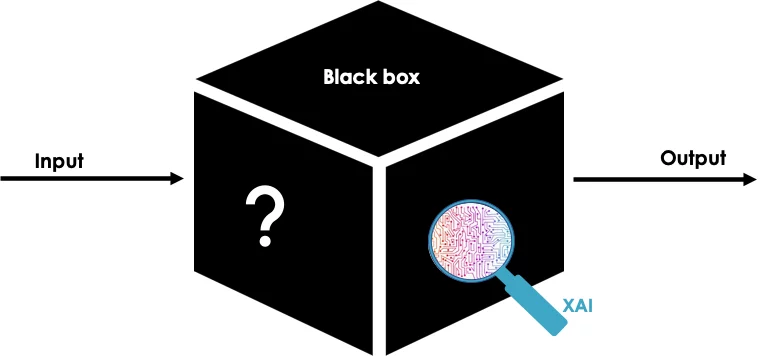
\includegraphics[scale=0.4]{TemplateTesi/immagini/blackboxpng.png}
    \caption{Problematica "Black Box" e uso della XAI \cite{imm_blackbox} }
    \label{fig:bb}
\end{figure}
Ad esempio, l'interpretazione dei modelli di AI potrebbe rivelare che determinate abitudini alimentari, personali o valori di alcune analisi influenzano significativamente la salute di un paziente. 
Queste informazioni possono aiutare i medici a consigliare cambiamenti specifici nello stile di vita, migliorando la salute complessiva dei pazienti



\end{flushleft}


